\documentclass[t]{beamer}
\usepackage[portuguese]{babel}
\usepackage[utf8]{inputenc}
\usetheme{Berkeley}
\usecolortheme{seahorse}

\addto\captionsportuguese{
	\renewcommand{\figurename}{Fig.}
	\renewcommand{\tablename}{Tab.}
}

\title{Micro processadores e controladores}
\subtitle{Suas características principais e sua importância para a área de IoT.}

\AtBeginSection[]
{
	\begin{frame}
	\frametitle{Sumário}
	\tableofcontents[currentsection]
\end{frame}
}

\begin{document}

\frame{\titlepage}

\begin{frame}
\frametitle{Sumário}
\tableofcontents
\end{frame}

\section{Componentes Básicos}

\begin{frame}{Componentes de um computador}
	\begin{itemize}
		\item CPU (Unidade Central de Processamento)
		\begin{itemize}
			\item Unidade de Controle
			\item Unidade Lógica/Aritmética
		\end{itemize}
		\item GPU (Unidade Gráfica de Processamento)
		\item Barramentos
		\item Clock
		\item Memória
		\item etc..
	\end{itemize}
\end{frame}

\section{Memórias}

\begin{frame}{Memórias}
	\begin{itemize}
		\item ROM
		\item PROM (programmable read-only memory)
		\begin{itemize}
			\item EPROM
			\item EEPROM
			\item UV-EPROM
		\end{itemize}
		\item FLASH
		\item RAM
		\begin{itemize}
			\item SRAM, Cache
			\item DRAM
		\end{itemize}
	\end{itemize}
\end{frame}

\section{Arquiteturas}

\begin{frame}{Arquiteturas}
	\begin{itemize}
		\item Von Neumann
		\begin{itemize}
			\item Dados e Programas na memória
			\item Compacta
		\end{itemize}
		\item Harvard
		\begin{itemize}
			\item Memória separada para Dados e Programas
			\item Mais componentes
		\end{itemize}
	\end{itemize}
\end{frame}

\begin{frame}{Arquiteturas}
	Von Neumann
	
	\begin{figure}
		\includegraphics[width=\linewidth]{arquiteturavonneumann}
	\end{figure}
\end{frame}

\begin{frame}{Arquiteturas}
	Harvard
	\begin{figure}
		\includegraphics[width=\linewidth]{arquiteturaharvard}
	\end{figure}
\end{frame}

\begin{frame}{Arquiteturas}
	Comparação
	\begin{columns}
		\begin{column}{0.5\linewidth}
			\begin{figure}
				\includegraphics[width=\linewidth]{learn_arduino_Von_Neumann}
				\caption{Von Neumann}
			\end{figure}
		\end{column}
		\begin{column}{0.5\linewidth}
			\begin{figure}
				\includegraphics[width=\linewidth]{learn_arduino_Harvard}
				\caption{Harvard}
			\end{figure}
		\end{column}
	\end{columns}
\end{frame}

\begin{frame}{Arquiteturas}
	Conjuntos de Instruções
	\begin{itemize}
		\item CISC (Complex Instruction Set Computer)
		\begin{itemize}
			\item Instruções podem durar vários ciclos do clock
			\item Melhor uso da RAM
			\item Exemplo: AMD e Intel x86
		\end{itemize}
		\item RISC (Reduced Instruction Set Computer)
		\begin{itemize}
			\item Instruções são executadas em um ciclo de clock
			\item Uso intenso da RAM
			\item Exemplo: ARM e SPARC
		\end{itemize}
	\end{itemize}
\end{frame}

\section{Processamento}

\begin{frame}{Processamento de dados}
	Características
	\begin{itemize}
		\item Arquiteturas
		\item Memórias
		\item Clock
		\item BUS
		\item Interrupções
	\end{itemize}
\end{frame}

\begin{frame}{O que é um micro-processador?!}
	\begin{itemize}
		\item Criado em 1971: Intel 4004
		\item Única CPU
		\item Utiliza-se de recursos externos (memória, I/O)
		\item Pode fazer parte de um processador multi-core
		\item Baseia-se na arquitetura Von Neumann
	\end{itemize}
\end{frame}

\begin{frame}{Intel 4004}
	\begin{figure}[ht]
		\begin{minipage}[b]{0.45\linewidth}
			\centering
			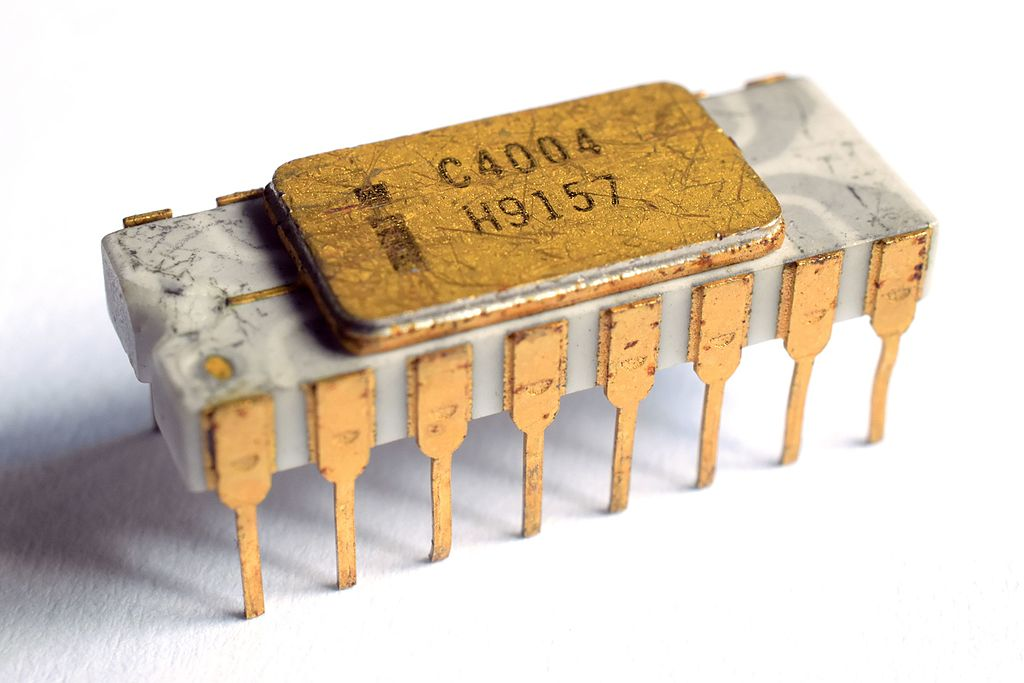
\includegraphics[width=0.9\textwidth]{Intel_C4004}
			\caption{Intel 4004 por fora}
		\end{minipage}
		\hspace{0.5cm}
		\begin{minipage}[b]{0.45\linewidth}
			\centering
			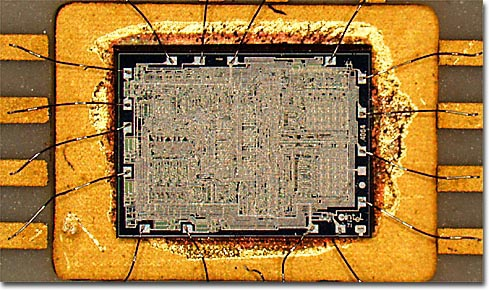
\includegraphics[width=0.9\textwidth]{Intel_C4004_die}
			\caption{Intel 4004 por dentro}
		\end{minipage}
	\end{figure}
\end{frame}

\begin{frame}{O que é um micro-controlador?!}
	\begin{itemize}
		\item Criado em 1971: TMS 1000
		\item Computador em um Chip
		\item Tem vários recursos internos (memória, I/O)
		\item Pode ser usado em sistemas embarcados 
		\item Baseia-se na arquitetura Harvard
	\end{itemize}
\end{frame}

\begin{frame}{TMS 1000}
	\begin{figure}[ht]
		\begin{minipage}[b]{0.45\linewidth}
			\centering
			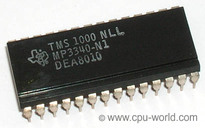
\includegraphics[width=0.9\textwidth]{TMS1000}
			\caption{TMS 1000 por fora}
		\end{minipage}
		\hspace{0.5cm}
		\begin{minipage}[b]{0.45\linewidth}
			\centering
				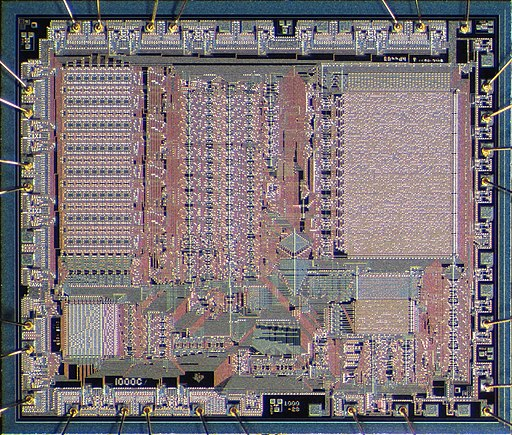
\includegraphics[width=0.9\textwidth]{TMS1000C_die}
			\caption{TMS 1000 por dentro}
		\end{minipage}
	\end{figure}
\end{frame}

\section{Pinagem}

\begin{frame}{Pinagem dos micro-controladores}
\begin{itemize}
\item Vin - Voltage input
\item GND - Ground
\item RST - Reset
\item CLK - Clock
\item RX - Receive
\item TX - Transmit
\item GPIO - General Purpose Input/Output
\item I2C - Inter-Integrated Circuit
\end{itemize}
\end{frame}

\section{Exemplos}

\begin{frame}{Exemplos}
Micro-processadores
\begin{itemize}
\item Intel
\begin{itemize}
\item Quark SoC
\end{itemize}
\item Broadcom
\begin{itemize}
\item BCM2835 SoC
\end{itemize}
\item Arm
\begin{itemize}
\item ARM11
\item Cortex A8, A15, A20
\end{itemize}
\end{itemize}
\end{frame}

\begin{frame}{Exemplos}
Micro-controladores
\begin{itemize}
\item Arduino
\item Atmel AVR
\item PIC (Microchip Technology)
\end{itemize}
\end{frame}

\begin{frame}{Exemplos}
Arquitetura do Arduino
\begin{figure}
\includegraphics[width=\linewidth]{Arduino-Architecture}
\end{figure}
\end{frame}

\begin{frame}{Exemplos}
ATMega 328 - Diagrama de blocos
\begin{figure}
\includegraphics[width=\linewidth]{atmega328-blockdiagram}
\end{figure}
\end{frame}

\begin{frame}{Exemplos}
	Detalhes da Arquitetura do Arduino UNO
	\begin{figure}
		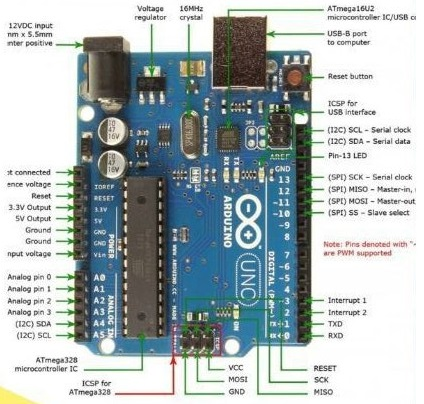
\includegraphics[width=0.7\linewidth]{arduino-uno-board}
	\end{figure}
\end{frame}

\begin{frame}{Exemplos}
Placas
\begin{itemize}
\item Raspberry Pi
\item Cubieboard
\item BeagleBone
\item NVidia
\end{itemize}
\end{frame}

\begin{frame}{Exemplos}
	Detalhes da Arquitetura do Raspberry Pi B+
	\begin{figure}
		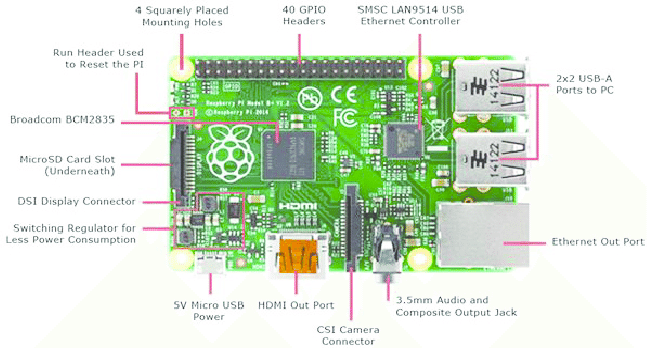
\includegraphics[width=\linewidth]{Raspberry-pi-B-model}
	\end{figure}
\end{frame}


\begin{frame}{Exemplos}
	Detalhes da Arquitetura do Raspberry 4
	\begin{figure}
		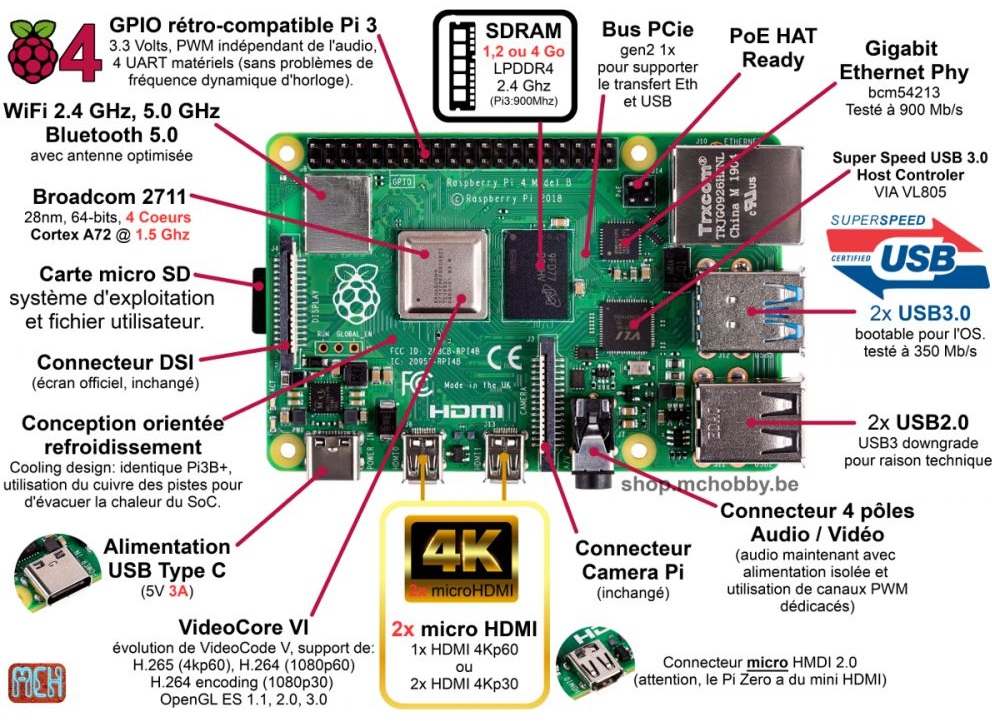
\includegraphics[width=0.8\linewidth]{raspberry-pi-4}
	\end{figure}
\end{frame}

\frame{\titlepage}

\end{document}
